\documentclass[10pt, oneside]{article}   	
\usepackage[margin=0.8in]{geometry}  
\usepackage[dvips]{graphics}
\usepackage{epsfig}
\usepackage{amsmath}
\usepackage{xspace}
\usepackage{fancybox}
\usepackage{graphicx,xspace,cite,verbatim,comment}
\usepackage[demo]{graphicx}
\usepackage{caption}
\usepackage{subcaption}
\usepackage{hyperref,array,color,balance,multirow}
\usepackage{balance,float,url,amsfonts,alltt}
\usepackage{mathtools,rotating,amsmath,amssymb}
\usepackage{color,cite,ifpdf,fancyvrb,array,listings}
\usepackage{algorithm,algpseudocode}
\usepackage{tabularx}
\usepackage{natbib}              		
\geometry{letterpaper}                   		
\usepackage{graphicx}		
\usepackage{subcaption}		
\usepackage{amssymb}

%SetFonts

%SetFonts


\title{\textbf{CS 638 Project Stage 2 Report}}
\author{Zhiwei Fan\hspace{7ex}
	   Lingfeng Huang\hspace{7ex}
	   Fang Wang\\
	   zfan29@wisc.edu\hspace{3ex}
	   lhuang58@wisc.edu\hspace{3ex}
	   fwang64@wisc.edu
	   }
%\date{}							% Activate to display a given date or no date

\begin{document}
\maketitle 

\section*{Source Websites and Relevant Documentation}
\begin{enumerate}
  	\item Source Websites:\\
		\textbf{Barnes\&Noble}: \textit{http://www.barnesandnoble.com}\\
		\textbf{Goodreads}: \textit{https://www.goodreads.com}
		
	\item Corresponding Tables:\\
		\textbf{tableA.csv}: table transformed from \textbf{Barnes\&Noble}'s data\\
		\textbf{tableB.csv}: table transformed from \textbf{Goodreads}'s data
		
	\item Original Schema:\\
		\textbf{tableA}(\underline{id}: integer, title: string, year: integer, pages: integer, day: integer, publisher: string, month: integer, authors: string, ISBN13: string)\\
		\textbf{tableB}(\underline{id}: integer, title: string, isbn: string, pageCount: integer, author: string, publisher: string, date: string)	
\end{enumerate}

\section*{Schema Transformation}
According to \textit{Original Schema} in previous section, tableA and tableB originally have different schemas. After careful consideration, we decide to transform both tables to 
be in the consistent schema shown as the following: 
\vspace{1ex}
 \\
 \textbf{table}(\underline{id}: integer, title: string, authors: string, ISNB13: string,  pages: integer, publisher: string, publishedYear: integer, publishedMonth: integer, publishedDay: integer,)
 
 \subsection*{Specific Steps of Transformation}
 Most attributes in \textit{tableA} remain the same. The only change made to \textit{tableA} was that \textit{ISBN3} was renamed to be \textit{isbn3},
 \textit{year} was renamed to \textit{publishedYear},  \textit{month} to \textit{publishedMonth}, \textit{day} to \textit{publishedDay}. For \textit{B}
 the attribute \textit{isbn} was renamed to \textit{isnb3}, \textit{pageCount} was renamed to \textit{pages}; attribute \textit{date} has been properly 
 parsed and split into three separated attributes \textit{publishedYear}, \textit{publishedMonth} and \textit{publishedDay} by running appropriate python scripts on the original csv files \textit{tableA.csv} 
 and \textit{tableB.csv} (additional \textit{reordering} has also been done to further strengthen the consistence and make it more convenient when coming to the data analysis and cleaning stage).
 
 \subsection*{Set of Attribute: S}
 According to the transformation steps we have described in the previous part, the attributes of the consistent schema in \textit{set S} is: \\
\textit{ id, title, authors, ISBN13, pages, publisher,  publishedYear, publishedMonth, publishedDay}.


\section*{Attributes Analysis (Table A)}
We take Table A as example to show our analysis of attributes. The same process and ideas have been applied to Table B as well. Due to the space limitation, we omit the analysis of 
Table B here and only display our results for Table A. 
\subsection*{Missing Values}
In Table A, there are only three attributes we have detected with \textit{missing value} issue and there are: \textit{pages}, \textit{publishedDay}, \textit{authors}. The corresponding 
missing value statistical data is reported in the following subsection.

\subsubsection*{Relevant Statistical Data}
\textit{pages}:\\ 
\textbf{number of missing values}: 466\\ 
\textbf{missing percentage}: 8.83\%\\ 
\textbf{missing fraction}: 466/5279 

\vspace{1ex}
\noindent
\\
\textit{publishedDay}: \\
\textbf{number of invalid values}: 4 \\ 
\textbf{missing percentage}: 0.75\% 
\textbf{missing fraction} 4/5279

\vspace{1ex}
\noindent
\\
\textit{authors}: \\
\textbf{number of missing values}: 2 \\ 
\textbf{missing percentage}: 0.39\% \\
\textbf{missing fraction}: 2/5279

\vspace{1ex}
\noindent
\\
Instead of using \textit{missing values}, we use \textit{invalid values} for attribute in \textit{publishedDay} for missing-value report. We do have found that every tuple in table A has attribute value 
\textit{publishedDay}, however, it's very obvious that some of those values are \textit{out of range} ( less than 1 or greater than 31). We regard these \textit{invalid values}
equivalent to \textit{missing values}.    

\subsubsection*{Discussion about Possible Solutions for Missing Values}
For those values are missing in \textit{pages}, the most naive way we could think is to fill `0' for every entry that \textit{page} is missing. However, this simple solution might not 
be feasible if \textit{pages} is considered as an important attribute when doing entity matching. Then there is high possibility we will \textit{miss} the match for those books that 
have `0' pages. The more complicated and tedious solution would be going to a few other websites, fetching the pages information again for those books that have missing values. Taking this
solution could give us much more reliable ``data fixing'' but will bring much more tedious work and put us under the risk of ``new data cleaning" task for those new data (which
is only used for fixing the \textit{real data} actually). For those values are missing in publishedDay and authors, since the number of values is very small, we could easily fix them
by searching the information on the source website we used for crawling data and fill those missing values manually in a few minutes. The decision of our final solution for missing 
values needs to be carefully considered based on both of the easiness of work and its influence on entity matching quality. 

\subsection*{Attributes Type Identification}
As shown in the schema of table in \textit{schema transformation} section, the attributes we have selected are all quite easy to determine their types:
\vspace{1ex}
\\
\textit{id}: integer, \textit{title}: string, \textit{authors}: string, \textit{ISNB3}: string,  \textit{pages}: integer, \textit{publisher}: string, \textit{publishedYear}: integer, \textit{publishedMonth}: integer, \textit{publishedDay}: integer
\vspace{1ex}
\\
\textit{publishedYear} , \textit{publishedMonth} and \textit{publishedDay} all have clear meaningful numerical domains and thus are identified as \textit{integer}. Every books's \textit{ISBN3} is composed of 13 numbers, which is not in the integer type value range  -2,147,483,648 to 2,147,483,647. Thus we identify \textit{ISBN3} as string type instead.
The number of total books could perfectly fit in the integer type value range, so we identify \textit{id}, the attribute we generated during the data crawling stage, as integer type.
\textit{title} and \textit{authors} are intuitively identified as string type and \textit{pages} is identified as integer type.

\subsection*{Textual Attribute Value Length Statistical Data Report}
There are \textit{four} textual attributes: \textit{title}, \textit{authors}, \textit{publisher}, \textit{ISBN3}
\vspace{0.5ex}
\\
\textit{title}: \\
\textbf{maximal length}: 255\\
\textbf{minimal length}: 4\\
\textbf{average length}: 67.078
\vspace{0.5ex}
\\
\textit{authors}:\\ 
\textbf{maximal length}: 193\\
\textbf{mininimal length}: 2\\
\textbf{average length}: 25.366
\vspace{0.5ex}
\\
\textit{publisher}:\\ 
\textbf{maximal length}: 60\\
\textbf{minimal length}: 3\\
\textbf{average length}: 19.64
\vspace{0.5ex}
\\
\textit{ISBN3}:\\ 
\textbf{maximal length}: 12\\
\textbf{minimal length}: 13\\
\textbf{average length}: 13

\subsection*{Possible Outliers and Anomalies Detection and}
\begin{figure}[H]
   \centering
   \begin{subfigure}{0.4\textwidth}
   	\centering
   	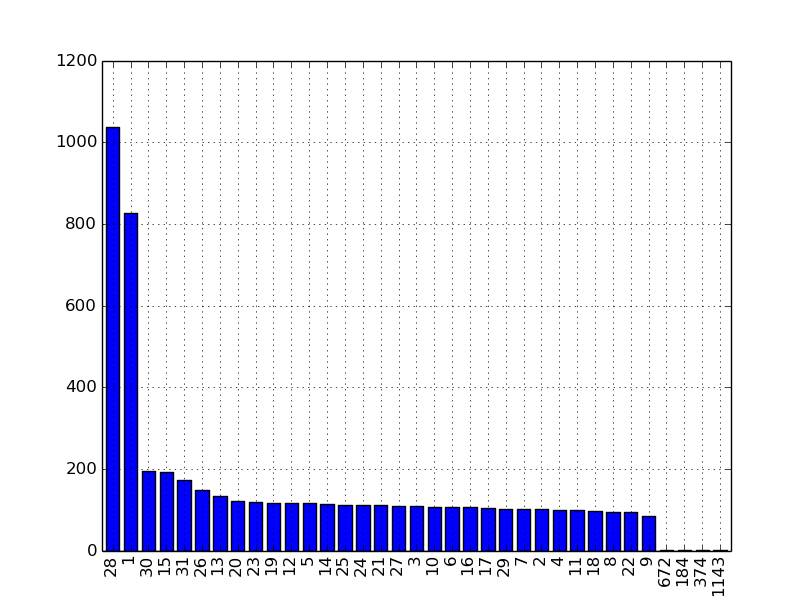
\includegraphics[height = 5cm]{publishedDay.png}  
   	\caption{Histogram on publishedDay values}
  	 \label{fig:publishedDay}
   \end{subfigure}
   \begin{subfigure}{0.4\textwidth}
   	\centering
   	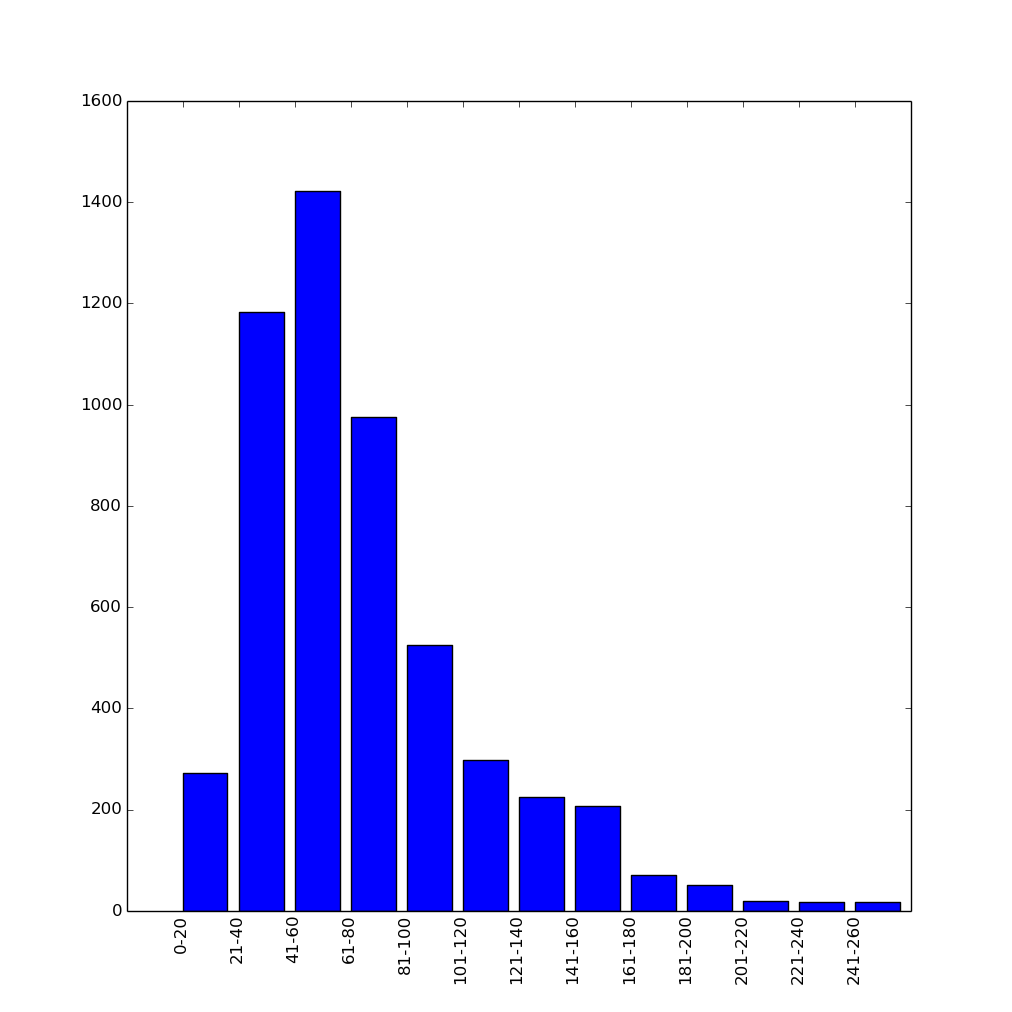
\includegraphics[height = 5cm]{title.png}  
   	\caption{Histogram on length of title values}
  	 \label{fig:title}
   \end{subfigure}
   \caption{Histograms for Anomaly Attribute Values Detection}
\end{figure}
We choose to use the analysis of attribute values of \textit{publishedDay} and \textit{title} to show our analysis on outliers detection. From figure \ref{fig:publishedDay},
extremely dense distribution on value 1 and 28 has been detected. Although we admit this \textit{extremely} high dense distribution is somehow different from 
the normal conception of \textit{outliers} (not attribute value anomaly), we think this observation is important since there might be high possibility of data corruptions 
(those publishedDays filled with \textit{1} and \textit{28} might not be exactly correct). In addition, we have also observed several \textit{outliers} according to the 
normal definition: \textit{672, 184, 374, 1143} are definitely \textit{out of range}. One possibility is that attribute values of other attributes have been incorrectly 
fetched and filled in the \textit{publishedDay} field. \textit{pages} is very likely to be in those attributes. One possible reason could be that the source websites
we used to crawling data from have accidentally mis-placed those values in the wrong place in their website structure. From figure \ref{fig:title}, we have observed 
that there are very few attribute values reside in the range 200 to 260, thus we conclude those values as possible outliers due to their low frequency and the big 
gap between those values and the average value of title length (67.078 according to \textit{Textual Attribute Value Length Statistical Data Report}).

\subsection*{Attribute Standard Discussion}
We intend to represent the published date of every book in \textit{year, month, day} separately. Originally, the published date is represented as a whole string in 
table B. We have already transform it into \textit{publishedYear, publishedMonth, publishedDay} as described in \textit{Specific Steps of Transformation}. All other 
attributes have intuitive and simple standard attribute value format as shown in the schema.
\subsection*{Synonyms Among Attribute Values Discussion}
Fortunately, \textit{synonyms} is unlikely to happen among attribute values of any attribute in our final schema. \textit{synonyms} are more likely to be seen in 
\textit{categorical attributes} and there is no categorical attributes in our schema.

\subsection*{Attribute Values Sprinkle Issues}
We do have found that for some tuples, attribute values are \textit{sprinkled} all over the item. For example, we have found that some tuples missed \textit{pages},
\textit{publisher}, \textit{publishedYear}, \textit{publishedMonth} and \textit{publishedDay} and those missing values actually show in \textit{title}. The result of this issue
result in both \textit{value missing} and \textit{outliner} (e.g., \textit{title} becomes long since it includes other \textit{wrong positioned attribute values}), which will 
further influence the \textit{entity matching} stage. The reason for this issues might be attributed the possibility that the source website we crawled data from have 
mis-positioned some attributes for some books or the lack of consideration of data structure and organization when crawling the data.

\subsection*{Additional Data Quality Problems}
Due to the \textit{data missing} and \textit{attribute values sprinkle issues}, some other data issues have also arisen and detected. For example, some attribute values
of some tuples have been detected to be placed in the \textit{wrong position}. This is either because of some attribute values before the \textit{misplaced attribute} 
have been missing or some previous values have been \textit{sprinkled} in other attributes.

\section*{Software Tools Used in Analysis and Data Cleaning}
We mainly used \textit{pandas} for data analysis (e.g., collecting information about missing values, length of title attribute, etc). In addition, we have used \textit{csv package} 
in \textit{python} to do relevant schema transformation and partial data cleaning.  



\end{document}  